\documentclass[aspectratio=169,11pt,t]{beamer}
% ============================================================
%  ksa-cs-v2: ksa-cs-lecture-template.tex 스타일 + 한글, v2 덱(16:9)용.
%    - 짙은 네이비 헤드라인 (섹션 이름 + 프레임마다 점)
%    - 꽉 찬 파란 제목 막대, 둥근 그림자 블록
%    - 한글: Noto Sans CJK KR (fontspec)
%  사용:
%    \documentclass[aspectratio=169,11pt,t]{beamer}
%    \input{<..>/theme/ksa-cs-v2.tex}
%  ksa-theme.tex 의 매크로(\kb \kq, ksablue/ksared 등)도 같은 이름으로 둔다
%  -> v2 덱 본문을 거의 그대로 옮길 수 있다.
% ============================================================

\usepackage{fontspec}
\usepackage{amsmath,amssymb}
\usepackage{tikz}
\usepackage{listings}
\usepackage{graphicx}
\usepackage{booktabs}
\usepackage{varwidth}
% enumitem 은 넣지 않는다 (beamer 글머리표가 사라진다)

\defaultfontfeatures{Ligatures=TeX}
\setmainfont{Noto Sans CJK KR}
\setsansfont{Noto Sans CJK KR}
\setmonofont{Noto Sans Mono CJK KR}[Scale=0.92]
\usefonttheme{professionalfonts}

% ---------- 기본 틀 ----------
\usetheme{default}
\useinnertheme[shadow=true]{rounded}
\setbeamertemplate{navigation symbols}{}
\setbeamersize{text margin left=1em,text margin right=1em}

% ---------- 색 (템플릿 원본 값) ----------
\definecolor{navydark}{HTML}{191959}
\definecolor{navydim}{HTML}{8888B0}
\definecolor{navytitle}{HTML}{262686}
\definecolor{navyblue}{HTML}{3333B2}
\definecolor{blockbodybg}{HTML}{E9E9F3}
\definecolor{examplegreen}{HTML}{006000}
\definecolor{examplebg}{HTML}{E5EFE5}
\definecolor{alertred}{HTML}{BF0000}
\definecolor{alertbg}{HTML}{F9E5E5}
% ksa-theme.tex 와 같은 이름 (본문 호환)
\colorlet{ksablue}{navytitle}
\colorlet{ksabluedk}{navydark}
\definecolor{ksagold}{HTML}{D6CBB1}
\definecolor{ksagolddk}{HTML}{A9976B}
\colorlet{ksared}{alertred}
\definecolor{ksagray}{HTML}{5B5B5B}

\setbeamercolor{structure}{fg=navyblue}
\setbeamercolor{alerted text}{fg=alertred}
\setbeamercolor{frametitle}{bg=navytitle,fg=white}
\setbeamercolor{title}{fg=white,bg=navytitle}
\setbeamercolor{block title}{bg=navytitle,fg=white}
\setbeamercolor{block body}{bg=blockbodybg,fg=black}
\setbeamercolor{block title example}{bg=examplegreen,fg=white}
\setbeamercolor{block body example}{bg=examplebg,fg=black}
\setbeamercolor{block title alerted}{bg=alertred,fg=white}
\setbeamercolor{block body alerted}{bg=alertbg,fg=black}
\setbeamercolor{item}{fg=navyblue}
\setbeamertemplate{itemize item}[circle]
\setbeamertemplate{itemize subitem}[triangle]

% ---------- 헤드라인: miniframes (섹션 이름 + 점) ----------
\useoutertheme[subsection=false]{miniframes}
\setbeamerfont{section in head/foot}{size=\tiny}
\setbeamercolor{section in head/foot}{bg=navydark,fg=white}
\setbeamercolor{mini frame}{fg=white}
\setbeamertemplate{mini frames}[circle]

% ---------- 제목 막대: 폭 꽉 채움, 두 줄까지 ----------
\setbeamerfont{frametitle}{size=\normalsize,series=\bfseries}
\setbeamertemplate{frametitle}{%
  \nointerlineskip
  \begin{beamercolorbox}[wd=\paperwidth,ht=2.7ex,dp=1.1ex,leftskip=.3cm,rightskip=.3cm]{frametitle}%
    \usebeamerfont{frametitle}\insertframetitle
  \end{beamercolorbox}}

% ---------- 쪽 번호: 오른쪽 아래 ----------
\setbeamertemplate{footline}{%
  \hfill
  {\color{navydim}\scriptsize\insertframenumber\,/\,\inserttotalframenumber}%
  \hspace{3mm}\vspace{2mm}%
}

% ---------- 표지: 템플릿처럼 헤드라인은 그대로, 가운데 둥근 그림자 상자에 제목 한 줄 ----------
% 덱에서:  {\setbeamertemplate{footline}{}\begin{frame}[c,noframenumbering]\titlepage\end{frame}}
\setbeamercolor{title}{fg=white,bg=navyblue}
\makeatletter
\setbeamertemplate{title page}{%
  \vfill
  \centering
  \begin{minipage}{0.84\paperwidth}
  \begin{beamercolorbox}[wd=\linewidth,sep=7pt,center,rounded=true,shadow=true]{title}
    {\usebeamerfont{title}\inserttitle\par}%
    \ifx\insertsubtitle\@empty\else\vskip0.4em{\usebeamerfont{subtitle}\insertsubtitle\par}\fi
  \end{beamercolorbox}
  \end{minipage}\par\vskip1.6em
  {\usebeamerfont{author}\color{navytitle}\insertauthor\par}\vskip0.3em
  {\usebeamerfont{institute}\color{ksagray}\insertinstitute\par}
  \vfill
}
\makeatother
\setbeamerfont{title}{series=\bfseries,size=\Large}
\setbeamerfont{subtitle}{size=\normalsize}
\setbeamerfont{author}{size=\normalsize}
\setbeamerfont{institute}{size=\small}

% ksa-theme 호환: 덱이 \renewcommand{\ksacredit}{..} 를 해도 되게 (꼬리말에는 안 쓴다)
\newcommand{\ksacredit}{}

% ---------- 강조 ----------
\newcommand{\hl}[1]{\textcolor{alertred}{#1}}
\newcommand{\hlb}[1]{\textcolor{navyblue}{#1}}
\newcommand{\kb}[1]{\textbf{\color{ksablue}#1}}
\newcommand{\kq}[1]{\textbf{\color{ksared}#1}}

% ---------- 파이썬 코드 (템플릿과 같은 색) ----------
\definecolor{codekw}{HTML}{0033B3}
\definecolor{codebuiltin}{HTML}{BF0000}
\definecolor{codestr}{HTML}{067D17}
\definecolor{codecomment}{HTML}{8C8C8C}
\definecolor{codenum}{HTML}{1750EB}
\lstdefinestyle{py}{
  language=Python, basicstyle=\ttfamily\scriptsize,
  keywordstyle=\color{codekw}\bfseries, stringstyle=\color{codestr},
  commentstyle=\color{codecomment}\itshape, numberstyle=\color{codenum},
  emph={print,len,range,sum,input,int,str,float,list,dict,append,remove,sorted,abs,min,max},
  emphstyle=\color{codebuiltin}, showstringspaces=false, keepspaces=true,
  columns=fixed, basewidth=0.52em, aboveskip=1mm, belowskip=1mm, xleftmargin=2mm,
  breaklines=true
}
\lstset{style=py}

% 원본 덱 (ksa-theme): slides/v2/ml1/week06/train_val_test/ -- 그림은 거기 figs/ 를 그대로 쓴다
\setbeamerfont{author}{size=\normalsize}
\setbeamerfont{institute}{size=\small}
\graphicspath{{../../../v2/ml1/week06/train_val_test/figs/}{../../../assets/}}
\makeatletter
\newcommand{\markpage}[1]{\protected@write\@auxout{}{\string\newlabel{#1}{{\the\c@framenumber}{}}}\hypertarget{#1}{}}
\newcommand{\pref}[1]{\hyperlink{#1}{\textcolor{ksagolddk}{(p.\ref{#1})}}}
\makeatother

\renewcommand{\ksacredit}{Machine Learning and Deep Learning \,\textperiodcentered\, train / val / test 와 데이터 누수}
\title{train / val / test 와 데이터 누수}
\subtitle{시험 데이터는 마지막까지 손대지 않는다}
\author{Machine Learning and Deep Learning}
\institute{한국과학영재학교 (KSA)}
\date{}
\begin{document}
{\setbeamertemplate{footline}{}\begin{frame}[c,noframenumbering]\titlepage\end{frame}}

\section{질문}
% --- 오늘의 질문
\begin{frame}{오늘의 질문}
\vfill
\centering
{\Large 100명에게 \textbf{아무 뜻 없는 난수} 5,000개씩. 정답은 \textbf{동전 던지기}.}\\[1.2em]
{\LARGE 이 데이터로 동전 앞뒤를 맞히는 AI: \kq{교차 검증 정확도 87\%}}\\[1.2em]
{\large 찍으면 50\% 가 정상이다. \textbf{무엇이 잘못됐을까?}}
\vfill
\note{100명에게 아무 뜻 없는 난수를 5000개씩 줬습니다. 정답은 동전을 던져 정했습니다. 이 데이터로 동전 앞뒤를 맞힐 방법은 없습니다. 찍으면 50퍼센트가 정상입니다. 그런데 지난 시간에 배운 교차 검증까지 제대로 했는데 정확도가 87퍼센트가 나왔습니다. 무엇이 잘못됐을까요? 오늘은 이렇게 성능이 부풀려지는 실수, 데이터 누수를 다룹니다.}
\end{frame}

\section{세 데이터}
% --- 세 데이터
\begin{frame}{세 데이터의 역할}
\markpage{flow}
\vfill
\centering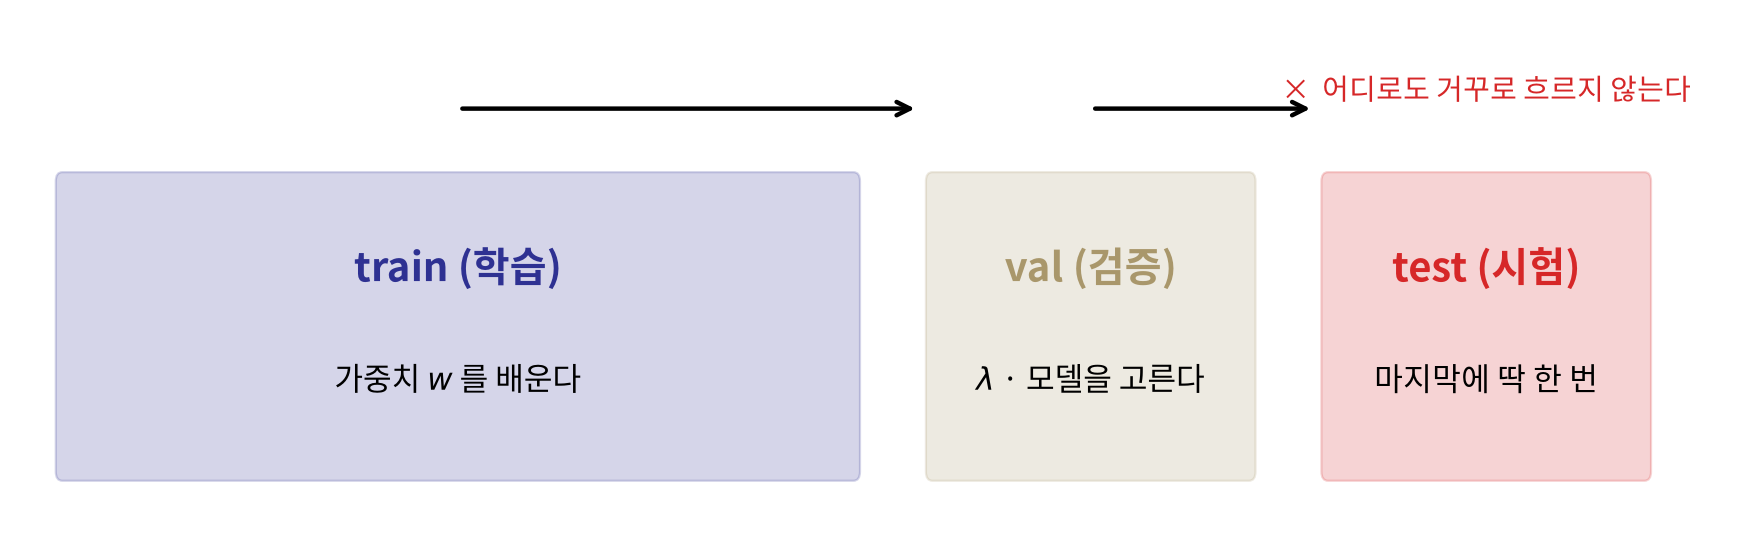
\includegraphics[width=0.86\linewidth]{tv_flow.png}\par\vskip0.3em
{\large 정보는 \textbf{train $\to$ val $\to$ test} 한 방향으로만 흐른다}\\[0.3em]
{\small val 은 교차 검증으로 대신할 수 있다 (train 안에서 돌아가며). test 는 \kq{따로 떼어 두고 마지막에 한 번}}
\vfill
\note{먼저 세 데이터의 역할을 정리합니다. train으로는 가중치를 배웁니다. val, 검증 데이터로는 람다 같은 설정값이나 여러 모델 중 하나를 고릅니다. 지난 시간처럼 train 안에서 돌아가며 교차 검증을 해도 됩니다. test, 시험 데이터는 모든 결정이 끝난 뒤 마지막에 딱 한 번 성능을 잽니다. 핵심은 정보가 한 방향으로만 흐른다는 겁니다. test의 정보가 어떤 식으로든 학습이나 선택으로 거꾸로 흘러 들어가면, test 점수는 더 이상 처음 보는 데이터의 성능이 아닙니다. 이것이 데이터 누수입니다.}
\end{frame}

% --- test 로 고르면
\begin{frame}{test 로 여러 번 고르면: 운이 점수에 섞인다}
\vfill
\centering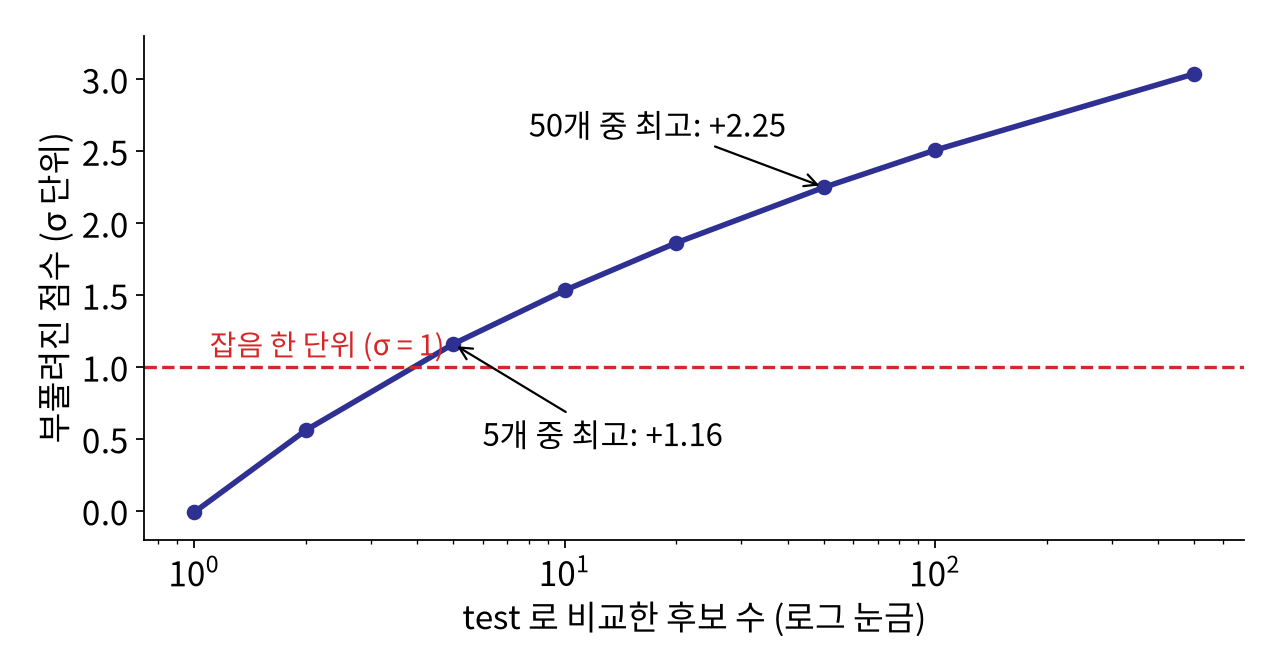
\includegraphics[width=0.56\linewidth]{tv_emax.png}\par\vskip0.2em
{\large 진짜 실력이 모두 같은 (0) 후보들을 test 로 비교해 최고를 고르면}\\[0.2em]
{\large 5개 중 최고: \kq{$+1.16\sigma$} \quad 50개 중 최고: \kq{$+2.25\sigma$} \quad $\to$ 후보가 많을수록 더 부풀려진다}
\vfill
\note{가장 흔한 누수는 test를 여러 번 보는 것입니다. 진짜 실력이 모두 똑같은 후보들을 test로 재면, 점수는 운에 따라 조금씩 위아래로 흔들립니다. 그중 가장 잘 나온 것을 고르면, 고른 점수는 진짜 실력보다 높을 수밖에 없습니다. 운이 좋았던 걸 골랐으니까요. 잡음 크기를 1로 두면, 후보 5개 중 최고는 평균 1.16만큼, 50개 중 최고는 2.25만큼 부풀려집니다. 람다 10개에 모델 5종류만 해도 후보가 50개입니다. 그래서 고르기는 val로 하고, test는 마지막에 한 번만 봅니다.}
\end{frame}

\section{누수}
% --- 누수 정의
\begin{frame}{데이터 누수 (Data Leakage)}
\vfill
\centering
{\LARGE 시험 데이터의 정보가 학습 과정에 \kq{몰래 새어 들어가는 것}}\\[1.2em]
\renewcommand{\arraystretch}{1.5}
{\large\begin{tabular}{rl}
1 & 고르기 · 전처리를 \textbf{전체 데이터}로 한 뒤에 나눈다\\
2 & 같은 \textbf{사람 (환자)} 의 데이터가 학습과 시험 양쪽에 들어간다\\
3 & \textbf{미래} 데이터로 학습하고 과거를 시험한다
\end{tabular}}\vskip0.6em
{\large 공통점: 실제로 쓸 때는 \textbf{없을} 정보를 시험 때 썼다}
\vfill
\note{데이터 누수는 시험 데이터의 정보가 학습 과정에 몰래 새어 들어가는 것입니다. 오늘은 세 가지 대표적인 경우를 봅니다. 첫째, 특징 고르기나 표준화 같은 전처리를 전체 데이터로 한 다음에 나누는 경우. 둘째, 같은 사람의 데이터가 학습과 시험 양쪽에 들어가는 경우. 셋째, 미래 데이터로 학습하고 과거를 시험하는 경우입니다. 공통점은 실제로 모델을 쓸 때는 없을 정보를 시험할 때 썼다는 것입니다.}
\end{frame}

% --- 동전 실험
\begin{frame}{누수 1: 전체 데이터로 특징을 고르면}
\markpage{coin}
\vfill
\centering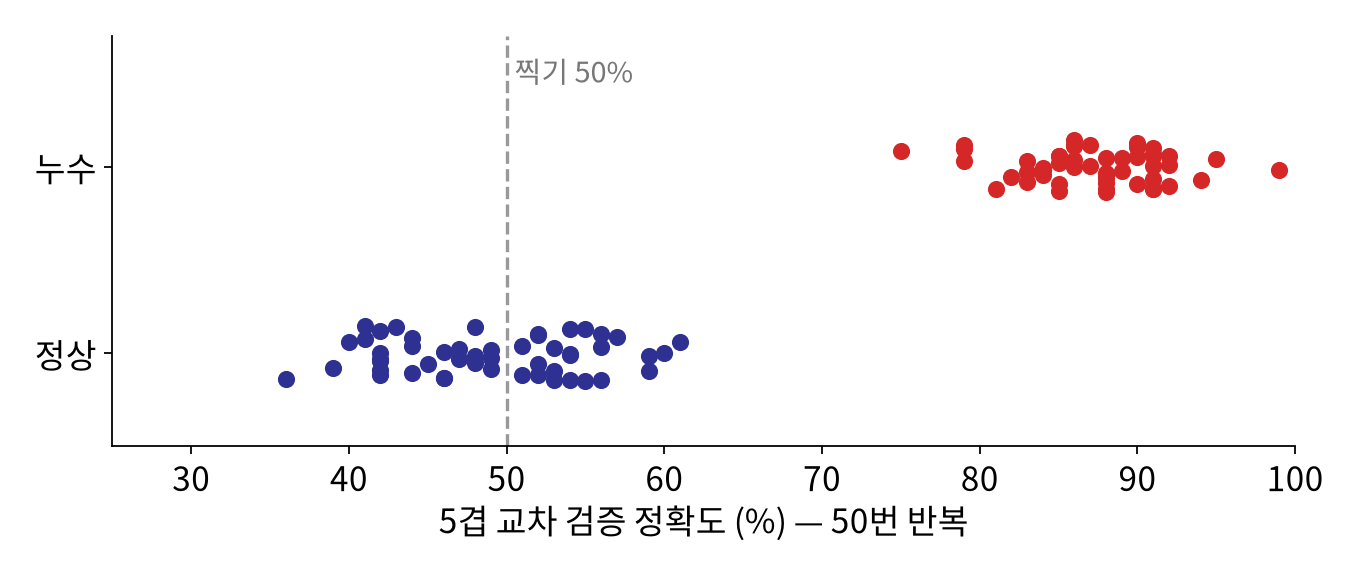
\includegraphics[width=0.64\linewidth]{tv_coin.png}\par\vskip0.2em
{\large \textbf{전체} 100명으로 숫자 20개를 고른 뒤 교차 검증 $\to$ \kq{87\%}}\\[0.2em]
{\large 고르기를 각 조각의 \textbf{학습 80명 안에서만} $\to$ \kb{49\%} \quad (찍기와 같다)}
\vfill
\note{처음의 동전 실험입니다. 범인은 숫자 고르기였습니다. 5000개 중 정답과 상관이 가장 큰 숫자 20개를 고를 때 100명 전체를 봤습니다. 시험 볼 학생까지 포함해서요. 5000개나 되면 우연히 정답과 맞아 보이는 숫자가 생기는데, 그 우연에는 시험 학생의 정답도 들어 있습니다. 그 숫자로 교차 검증을 하니 87퍼센트가 나왔습니다. 고를 때 이미 답을 본 셈입니다. 숫자 고르기를 각 조각의 학습 80명 안에서만 하면 49퍼센트, 찍기와 같습니다. 50번 반복해도 누수 쪽은 모두 75퍼센트 이상, 정상 쪽은 모두 61퍼센트 이하였습니다.}
\end{frame}

% --- 표준화 누수
\begin{frame}{누수 1: 표준화도 학습 데이터로만}
\vfill
\centering
{\large 데이터 1, 2, $\dots$, 10 \quad train = 1 $\sim$ 7, \quad test = 8, 9, 10}\vskip0.6em
\renewcommand{\arraystretch}{1.4}
{\Large\begin{tabular}{lccc}
평균 · 표준편차를 구한 곳 & 평균 & 표준편차 & test 의 $z$\\\hline
전체 1 $\sim$ 10 (\kq{누수}) & 5.5 & 2.872 & 0.87, 1.22, 1.57\\
train 1 $\sim$ 7 (\kb{정상}) & 4.0 & 2.0 & 2.0, 2.5, 3.0
\end{tabular}}\vskip0.6em
{\large test 는 사실 학습 범위 \textbf{밖}의 큰 값인데, 누수 통계로 보면 \kq{평범해 보인다}}\\[0.3em]
{\small 해결: 전처리도 모델의 일부 $\to$ train 으로 fit, val · test 에는 apply 만 (scikit-learn \texttt{Pipeline})}
\vfill
\note{특징 고르기만이 아닙니다. 표준화도 마찬가지입니다. 1부터 10까지 중 1에서 7을 train, 8, 9, 10을 test로 둡니다. 평균과 표준편차를 전체로 구하면 5.5와 2.872이고, test의 z는 0.87에서 1.57로 평범해 보입니다. train으로만 구하면 4와 2.0이고, test의 z는 2에서 3으로 학습 범위를 한참 벗어난 값이라는 게 드러납니다. 실제로 쓸 때는 새 데이터의 값을 미리 알 수 없으니 정상 쪽이 맞습니다. 전처리도 모델의 일부라고 생각하고 train으로만 fit하고, val과 test에는 apply만 합니다. scikit-learn의 Pipeline으로 묶으면 교차 검증 안에서도 자동으로 이렇게 됩니다.}
\end{frame}

% --- 환자 누수
\begin{frame}{누수 2: 같은 환자가 학습과 시험 양쪽에}
\markpage{patient}
\vfill
\centering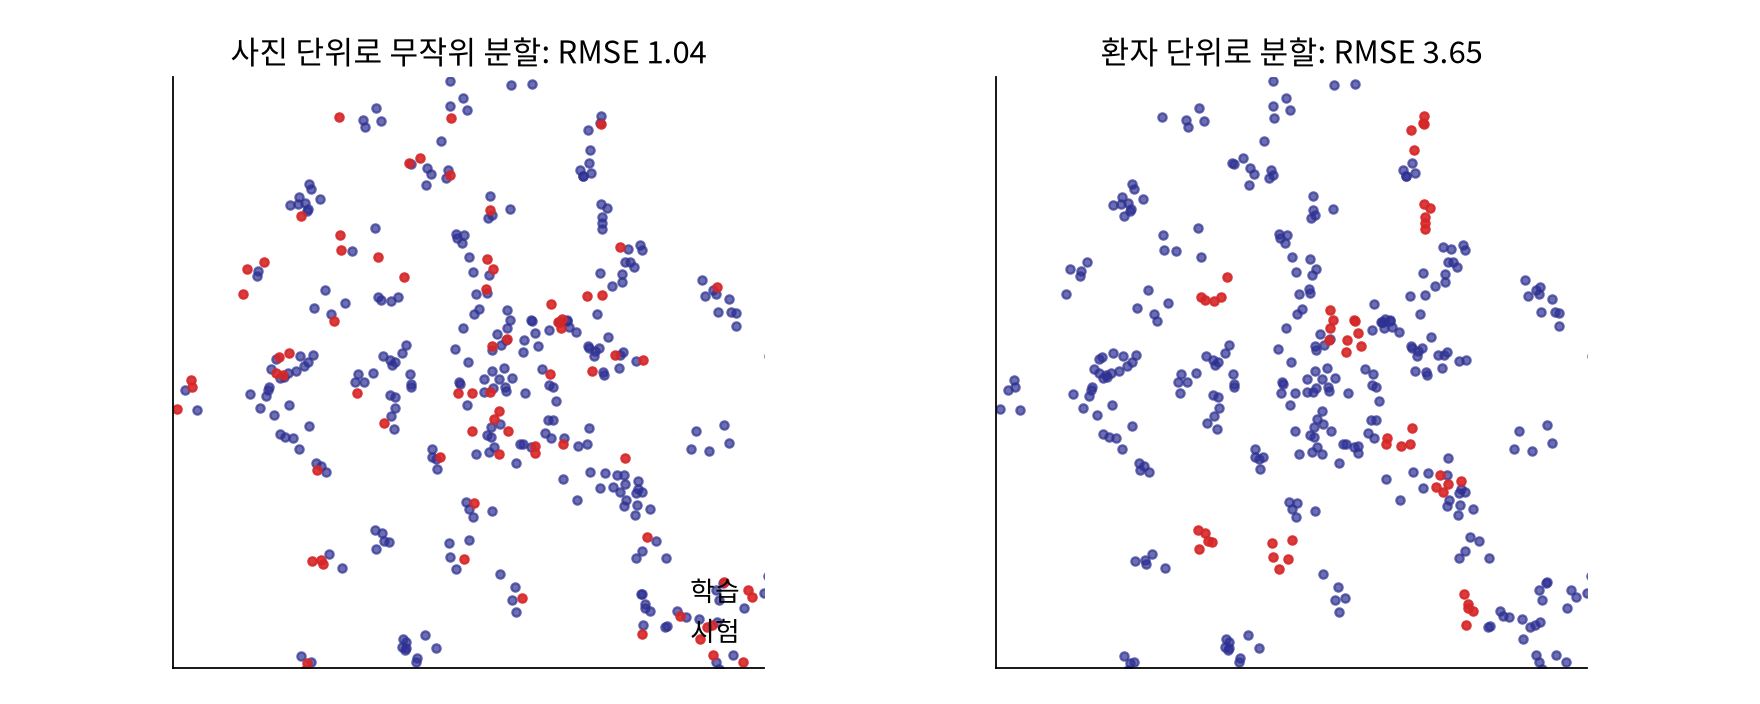
\includegraphics[width=0.76\linewidth]{tv_patient.png}\par\vskip0.2em
{\large 사진 단위로 섞으면 RMSE \kq{1.04} \quad 환자 단위로 나누면 \kb{3.65}}\\[0.2em]
{\small 환자 100명 × 사진 5장 (예시). 같은 환자의 다른 사진으로 맞힌 것 = 진단이 아니라 \textbf{환자 알아보기}}
\vfill
\note{두 번째는 의료 영상 AI에서 실제로 자주 발견되는 누수입니다. 환자 100명에게서 사진을 5장씩 찍었습니다. 한 환자의 사진 5장은 서로 아주 비슷해서 그림에서 작은 덩어리로 뭉쳐 있습니다. 사진 단위로 섞어서 나누면 왼쪽처럼 한 덩어리 안에 학습 사진과 시험 사진이 섞입니다. 그러면 모델은 같은 환자의 다른 사진을 보고 아 이 사람이네 하고 답을 맞힙니다. 오차가 1.04로 아주 좋아 보입니다. 환자 단위로 나눠서 시험 환자는 학습에 한 번도 안 나오게 하면 3.65가 됩니다. 이게 처음 보는 환자에게 쓸 때의 진짜 성능입니다. scikit-learn에서는 GroupKFold로 나눕니다.}
\end{frame}

% --- 시간 누수
\begin{frame}{누수 3: 미래로 과거를 맞히기}
\markpage{time}
\vfill
\centering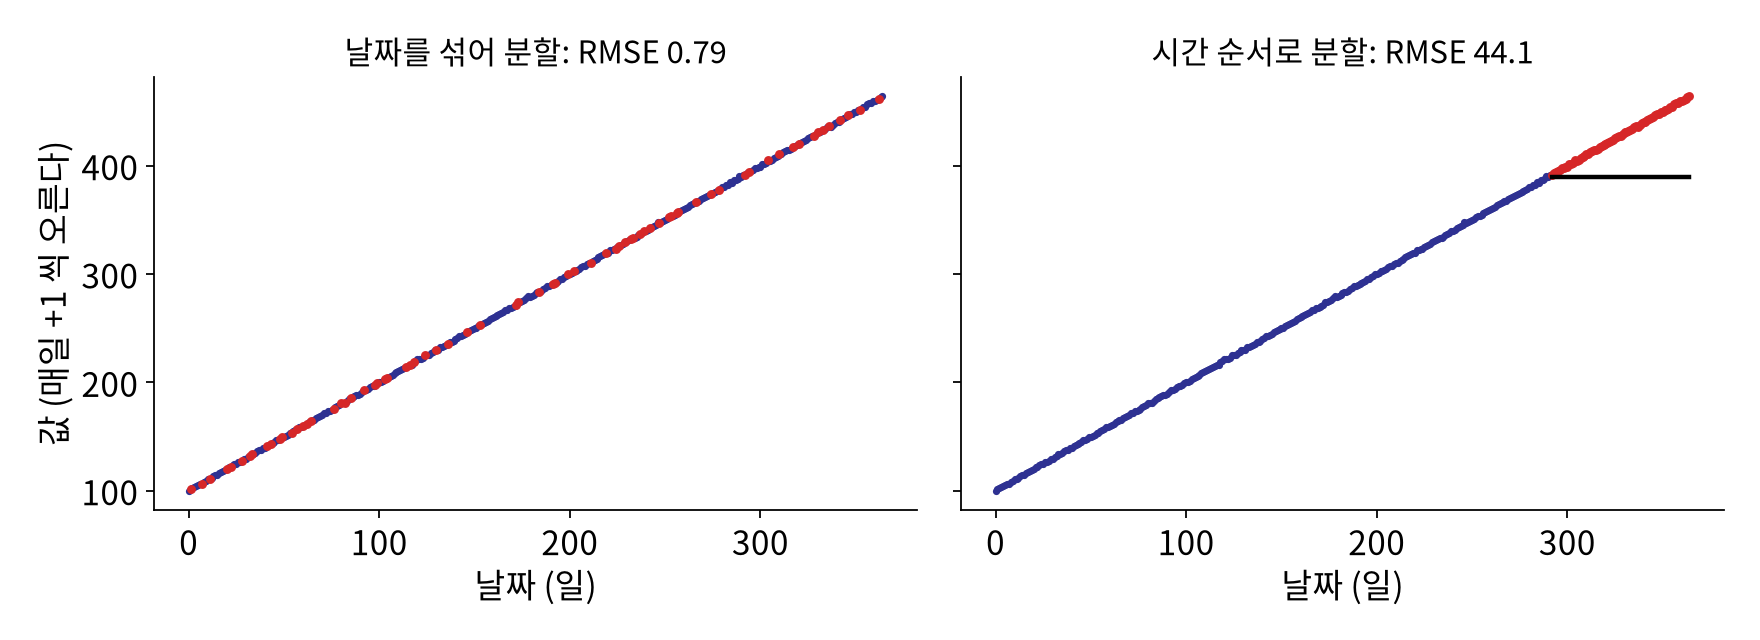
\includegraphics[width=0.76\linewidth]{tv_time.png}\par\vskip0.2em
{\large 날짜를 섞으면 RMSE \kq{0.79} \quad 시간 순서로 나누면 \kb{44.1}}\\[0.2em]
{\small 섞으면 시험 날짜 양옆이 학습 데이터라 사이만 메우면 된다. 실제 예측은 \textbf{내일}을 맞히는 일}
\vfill
\note{세 번째는 시간입니다. 매일 1씩 오르는 값을 1년 동안 쟀습니다. 날짜를 섞어서 나누면 시험 날짜 바로 어제와 내일이 학습 데이터에 있어서, 그 사이를 메우기만 하면 됩니다. 오차 0.79로 훌륭해 보입니다. 하지만 실제로 이 모델을 쓸 때는 내일을 예측해야 하고, 내일의 데이터는 없습니다. 앞 80퍼센트로 학습하고 뒤 20퍼센트를 시험하면, 모델은 학습 기간 끝의 값만 되풀이해서 오차가 44.1이 됩니다. 주가, 판매량, 센서처럼 시간 순서가 있는 데이터는 반드시 시간 순서로 나눕니다. scikit-learn에는 TimeSeriesSplit이 있습니다.}
\end{frame}

\section{규칙}
% --- 규칙
\begin{frame}{누수를 막는 규칙}
\vfill
\centering
\renewcommand{\arraystretch}{1.5}
{\normalsize\begin{tabular}{ll}
\textbf{test 를 제일 먼저 떼어 둔다} & 그래프 그리기보다도 먼저\\
\textbf{전처리 · 고르기는 train 으로만} & \texttt{Pipeline} 으로 묶는다\\
\textbf{단위를 지켜 나눈다} & 사람 · 환자 단위 (\texttt{GroupKFold})\\
\textbf{시간을 지켜 나눈다} & 과거로 학습, 미래로 시험 (\texttt{TimeSeriesSplit})\\
\textbf{test 는 딱 한 번} & 보고 다시 고치면 더 이상 test 가 아니다
\end{tabular}}\vskip0.6em
{\large 질문 하나로 점검: ``\textbf{실제로 쓸 때도 이 정보가 있을까?}''}
\vfill
\note{누수를 막는 규칙을 정리합니다. 데이터를 받으면 어떤 분석이나 그래프보다 먼저 test를 떼어 둡니다. 그래프를 보고 특징을 고르는 것도 정보가 새는 길이니까요. 표준화나 특징 고르기 같은 전처리는 train으로만 하고, Pipeline으로 묶어서 교차 검증 안에서 돌립니다. 같은 사람의 데이터는 같은 쪽에, 시간이 있는 데이터는 과거와 미래로 나눕니다. 그리고 test는 딱 한 번만 봅니다. 결과를 보고 모델을 다시 고치면 그 test는 이미 val이 된 겁니다. 헷갈릴 때는 실제로 모델을 쓸 때도 이 정보가 있을까라고 물어보면 됩니다.}
\end{frame}

% --- 전체 흐름
\begin{frame}{전체 흐름: 당뇨병 데이터 442명}
\vfill
\centering
\renewcommand{\arraystretch}{1.4}
{\large\begin{tabular}{rl}
1 & 나누기: train \textbf{265} · val \textbf{88} · test \textbf{89}\\
2 & 릿지 $\lambda$ 후보 5개를 train 으로 학습, val 로 비교 $\to$ $\lambda = 0.1$ (val RMSE 58.07)\\
3 & test 로 \textbf{한 번} 잰다 $\to$ test RMSE \kb{53.79} \quad 이 숫자를 보고한다\\
4 & (잘못) test 로 다시 고르면 $\to$ 그 숫자는 test 에서 운 좋은 값일 뿐
\end{tabular}}\vskip0.6em
{\small 숫자는 notebooks/ml1/chapter06\_3 과 같은 분할 (\texttt{random\_state=0})}
\vfill
\note{지금까지의 원칙을 실제 당뇨병 데이터 442명에 한 흐름으로 적용해 봅니다. 먼저 train 265명, val 88명, test 89명으로 나눕니다. 릿지 람다 후보 5개를 train으로 학습하고 val로 비교해서 0.1을 고릅니다. 그다음 test로 딱 한 번 재서 53.79가 나왔고, 이 숫자를 최종 성능으로 보고합니다. 만약 test 점수를 보고 람다를 다시 고르면, 그때 나온 숫자는 그 test에서 운 좋게 잘 나온 값일 뿐이라 정직한 성능이 아닙니다.}
\end{frame}

\section{연습}
% --- 문제풀이
\begin{frame}{문제풀이}
\vfill
\begin{enumerate}
\item 다음 중 누수인 것을 모두 고르라. \; (a) 전체 데이터로 결측치를 평균으로 채운 뒤 나눴다 \; (b) train 으로 구한 평균을 test 결측치에 채웠다 \; (c) 학생의 1학기 · 2학기 성적을 따로 행으로 두고 무작위로 나눴다\vskip0.8em
\item 내일 미세먼지를 예측하는 모델을 5겹 교차 검증 (섞음) 으로 평가했더니 아주 좋았다. 어떻게 다시 평가하겠나?\vskip0.8em
\item 같은 test 로 모델 20개를 비교해 가장 좋은 점수 92\% 를 보고했다. 무엇이 문제인가? 어떻게 고치나?
\end{enumerate}
\vfill
\note{1번 답. a는 test의 값이 평균에 섞였으니 누수입니다. b는 정상입니다. c는 같은 학생이 학습과 시험 양쪽에 들어갈 수 있으니 누수이고, 학생 단위로 나눠야 합니다. 2번 답. 시간 순서로 나눕니다. 예를 들어 과거 3년으로 학습하고 그다음 1년을 시험하거나, TimeSeriesSplit을 씁니다. 3번 답. 20개 중 최고를 고르면 운이 섞여 부풀려집니다. 고르기는 val이나 교차 검증으로 하고, 고른 모델 하나만 새 test로 한 번 잽니다.}
\end{frame}

% --- 실습
\begin{frame}{실습}
\vfill
\centering\begin{tabular}{rl}
\large 1 & 동전 실험 직접 해 보기: 전체로 고르기 vs \texttt{Pipeline} (찍기 근처로)\\[0.5em]
\large 2 & 환자 누수 · 시간 누수 재현: \texttt{GroupKFold}, \texttt{TimeSeriesSplit}\\[0.5em]
\large 3 & 당뇨병 3분할 파이프라인: val 로 고르고 test 는 한 번
\end{tabular}\vskip1em
Diabetes (Efron et al., 2004; scikit-learn) \\[0.4em]\href{https://colab.research.google.com/github/SuminHan/book-ml/blob/main/slides/v2/ml1/week06/train_val_test/lab/train_val_test.ipynb}{\textcolor{ksagolddk}{▶ Colab에서 실습 노트북 열기}}
\vfill
\note{실습은 세 부분입니다. 첫째, 동전 실험을 직접 해서 전체로 숫자를 고르면 90퍼센트 가까이 나오고, Pipeline으로 묶어 교차 검증 안에서 고르면 찍기 근처로 떨어지는 걸 확인합니다. 둘째, 환자 누수와 시간 누수를 재현하고 GroupKFold와 TimeSeriesSplit으로 고칩니다. 셋째, 당뇨병 데이터로 train, val, test 3분할 파이프라인을 처음부터 끝까지 해 봅니다.}
\end{frame}

\section{정리}
% --- 정리
\begin{frame}{정리}
\vfill
\centering\large\begin{tabular}{l}
train: 배우기 \quad val (교차 검증): 고르기 \quad \kq{test: 마지막에 한 번}\\[0.5em]
test 로 여러 번 고르면 운이 섞인다 (50개 중 최고 $+2.25\sigma$)\\[0.5em]
\textbf{누수}: 전체로 전처리 (87\% vs 49\%), 같은 환자 (1.04 vs 3.65), 미래 (0.79 vs 44.1)\\[0.5em]
``실제로 쓸 때도 이 정보가 있을까?''
\end{tabular}
\vfill
\note{정리합니다. train으로 배우고, val이나 교차 검증으로 고르고, test는 마지막에 한 번만 봅니다. test로 여러 번 고르면 운이 점수에 섞여 부풀려집니다. 데이터 누수는 전체 데이터로 전처리하기, 같은 환자를 양쪽에 넣기, 미래로 과거를 맞히기처럼 실제로는 없을 정보를 시험 때 쓰는 것이고, 오늘 본 것처럼 성능을 크게 부풀립니다. 헷갈리면 실제로 쓸 때도 이 정보가 있을까를 물어보세요.}
\end{frame}
\end{document}
